%----------------------------------------------------------------------------------------
%	PACKAGES AND THEMES
%----------------------------------------------------------------------------------------

\documentclass[12pt,presentation,notes]{beamer}
%\documentclass[12pt,presentation]{beamer}

\usetheme{default}
\usecolortheme{default}

%\useoutertheme{smoothbars}
\useinnertheme{rounded}

\setbeamertemplate{footline}{~\quad~\insertshorttitle~|~\insertshortauthor\hfill\insertsectionnumber.\insertsubsectionnumber~\insertsection\hfill\insertdate~\quad~
\begin{tikzpicture}
\draw node {\insertframenumber/\inserttotalframenumber};
\draw [black,very thick,domain=0:360] plot ({0.3*cos(\x)}, {0.3*sin(\x)});
\draw [MyTheme,very thick,domain=0:(360*\insertframenumber)/(\inserttotalframenumber))] plot ({0.3*cos(\x)}, {0.3*sin(\x)});
\end{tikzpicture}~\quad\quad\vspace{0.3cm}
}
\setbeamertemplate{navigation symbols}{}
\setbeamertemplate{section in toc}{\inserttocsectionnumber.~\inserttocsection}
\setbeamertemplate{subsection in toc}{\quad\inserttocsectionnumber.\inserttocsubsectionnumber~\inserttocsubsection \\}

\usepackage[T1]{fontenc}
\usepackage[default]{sourcesanspro}
\usepackage[utf8x]{inputenc}

\usepackage{graphicx}

\graphicspath{D:/LATEX/Reports@IIT/figures}

\usepackage{xcolor,colortbl}

\setbeamerfont{title}{series={\huge}}
\setbeamerfont{frametitle}{series={\bfseries}}
\setbeamerfont{block title}{series={\normalsize\bfseries}}
\setbeamertemplate{frametitle}{\begin{centering}\smallskip\insertframetitle\par\smallskip\end{centering}}
\setbeamertemplate{itemize items}{\tikz\node[draw=MyTheme, circle, very thick,fill=MyThemeLight,inner sep=0.08cm] {};}{}

\usepackage{pgf,tikz}
\usetikzlibrary{shapes.callouts}

\tikzset{
  level/.style   = { ultra thick, blue },
  connect/.style = { dashed, red },
  notice/.style  = { ultra thick, draw=MyTheme, rectangle callout, rounded corners, inner sep=1em,callout relative pointer={#1},fill=MyThemeLight },
  label/.style   = { text width=2cm }
}

%%%%%%%%%%%%%%%%%%%%%%%%%%%%%%%%%%%%%%%%%%%%%%%%%%%%%%%% Define some colors:
\definecolor{TuscanRed}    {HTML}{71283F}
\definecolor{DarkFern}     {HTML}{407428}
\definecolor{OceanBlue}    {HTML}{293F70}
\definecolor{DarkCharcoal} {HTML}{4D4944}

\colorlet{MyTheme}{DarkFern}
%\colorlet{MyTheme}{TuscanRed}
%\colorlet{MyTheme}{OceanBlue}
\colorlet{MyThemeLight}{MyTheme!30!white}

\colorlet{Charcoal}{DarkCharcoal!85!white}
\colorlet{LightCharcoal}{Charcoal!50!white}
\colorlet{AlertColor}{MyTheme}

\setbeamercolor{title}          {fg=black}
\setbeamercolor{frametitle}     {fg=black}
\setbeamercolor{normal text}    {fg=black}
\setbeamercolor{block title}    {fg=black,bg=MyTheme!70!white}
\setbeamercolor{block body}     {fg=black,bg=MyThemeLight}
\setbeamercolor{structure}      {fg=MyTheme}
\setbeamercolor{alerted text}   {fg=AlertColor}
\setbeamercolor{itemize item}   {fg=Charcoal}
\setbeamercolor{enumerate item} {fg=MyTheme}
%%%%%%%%%%%%%%%%%%%%%%%%%%%%%%%%%%%%%%%%%%%%%%%%%%%%%%%%%%%%%%%%%%%%%%%%%%%%%%%%%%%%%%%%%%%%%%%%%%%%%%%%%%%%%%%%%%%%%%%%%%%%%%%%%%

\title[Short Title]{Insert Title Here}
\author[PHIL101]{\normalsize Philosophy 101}
\institute{\normalsize Heartland Community College}
\date{\today}

\AtBeginSection[]
{
  \begin{frame}[plain]
    \frametitle{Outline for Section \thesection}
    \tableofcontents[currentsection]
  \end{frame}
}

\hyphenpenalty=10000000

\begin{document}

\usebackgroundtemplate{\tikz[overlay,remember picture]\node[opacity=0.3,at=(current page.center)] {\includegraphics[width=\paperwidth,height=\paperheight]{../bg/bg01}};}
\begin{frame}[plain]\vspace{1cm}\titlepage\end{frame}
\usebackgroundtemplate{}

\begin{frame}[plain]
\frametitle{Outline for Discussion}
\tableofcontents
\end{frame}


%%%%%%%%%%%%%%%%%%%%%%%%%%%%%%%%%%%%%%%%%%%%%%%%%%%%%%%%%%%%%%%%%%%%%%%%%%%%%%%%%%%%%%%%%%%%%%%%%%%%%%%%%%%%%%%%%%%%%%%%%%%%%%%%%%

\section{Intro}
\begin{frame}
\frametitle{Arc}

\insertframenumber/\inserttotalframenumber

\end{frame}

\subsection{Intro A}
\subsection{Intro B}


\begin{frame}
\frametitle{Kant on the Good Will}

\begin{tikzpicture}[overlay,remember picture]
 \node[notice={(1,-0.5)}, text width=6.5cm] at (3.5,0) {What makes a good will good? It isn't what it brings about, its usefulness in achieving some intended end. Rather, good will is good because of how it wills -- i.e. it is good in itself. Taken just in itself it is to be valued incomparably more highly than anything that could be brought about by it in the satisfaction of some preference -- or, if you like, the sum total of all preferences!};
 \node[] at (10,-1.5) {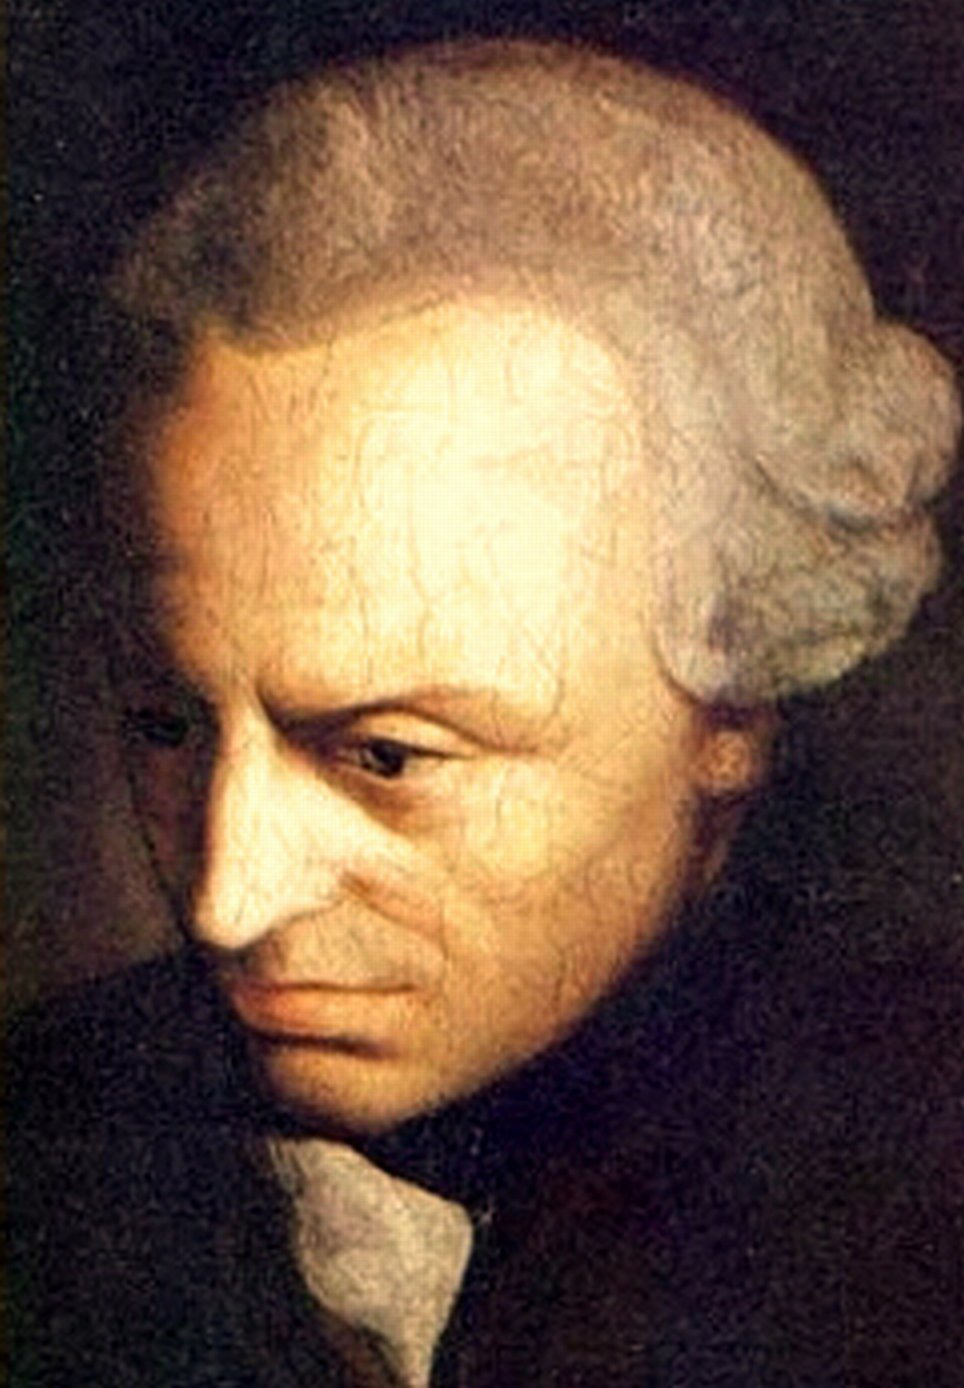
\includegraphics[width=3cm]{kant}};
\end{tikzpicture}

\end{frame}

\begin{frame}
\frametitle{Quiz Slide}

Which philosopher died by drinking tea made from poisonous hemlock?

\begin{enumerate}[\bfseries (A)]
\item<2-5> John Locke
\item<3-5> Immanuel Kant
\item<4-> \textbf<6>{\color<6>{MyTheme}Socrates}
\item<5-5> Susan Haack
\end{enumerate}

% Cool Specifications:
%   \textbf<1->{    controls when to bold text}
%   \textit<>{}    controls when to italicize text
%   \color<>[]{}   controls when to change color of text
%   \item<>        controls when an item is shown

%   \only<>{}      controls when to reveal text, occupies NO space otherwise
%   \uncover<>{}   controls when to reveal text, DOES occupy space otherwise
%   \alt<>{}{}     reveals first argument when specification is true, otherwise reveals second argument
%   \alert<>{}     controls when to highlight text (default red)

\end{frame}

\begin{frame}
\frametitle{Epicurus' Argument Against the Harmfulness of Death}

\begin{block}<1->{Premise 1}
We do not exist after death.
\end{block}
\begin{block}<2->{Premise 2}
If we do not exist after death, then being dead does not harm us.
\end{block}
\begin{block}<3->{Conclusion}
So, being dead does not harm us.
\end{block}

\end{frame}

\begin{frame}
\frametitle{Korman-Style Argument}


\begin{block}<1->{}
\textbf{\alert{(A1)}}\quad   \uncover<2->{We do not exist after death.}
\end{block}
\begin{block}<1->{}
\textbf{\alert{(A2)}}\quad   \uncover<3->{If we do not exist after death, then being dead does not harm us.}
\end{block}
\begin{block}<1->{}
\textbf{\alert{(A3)}}\quad   \uncover<4->{So, being dead does not harm us.}
\end{block}

\end{frame}


\subsection{Intro C}
\section{Middle A}
\section{Middle B}
\subsection{Middle B1}


\begin{frame}
\frametitle{Double Column Slide}
\begin{columns}
\column{0.35\textwidth}

\begin{figure}[HT]
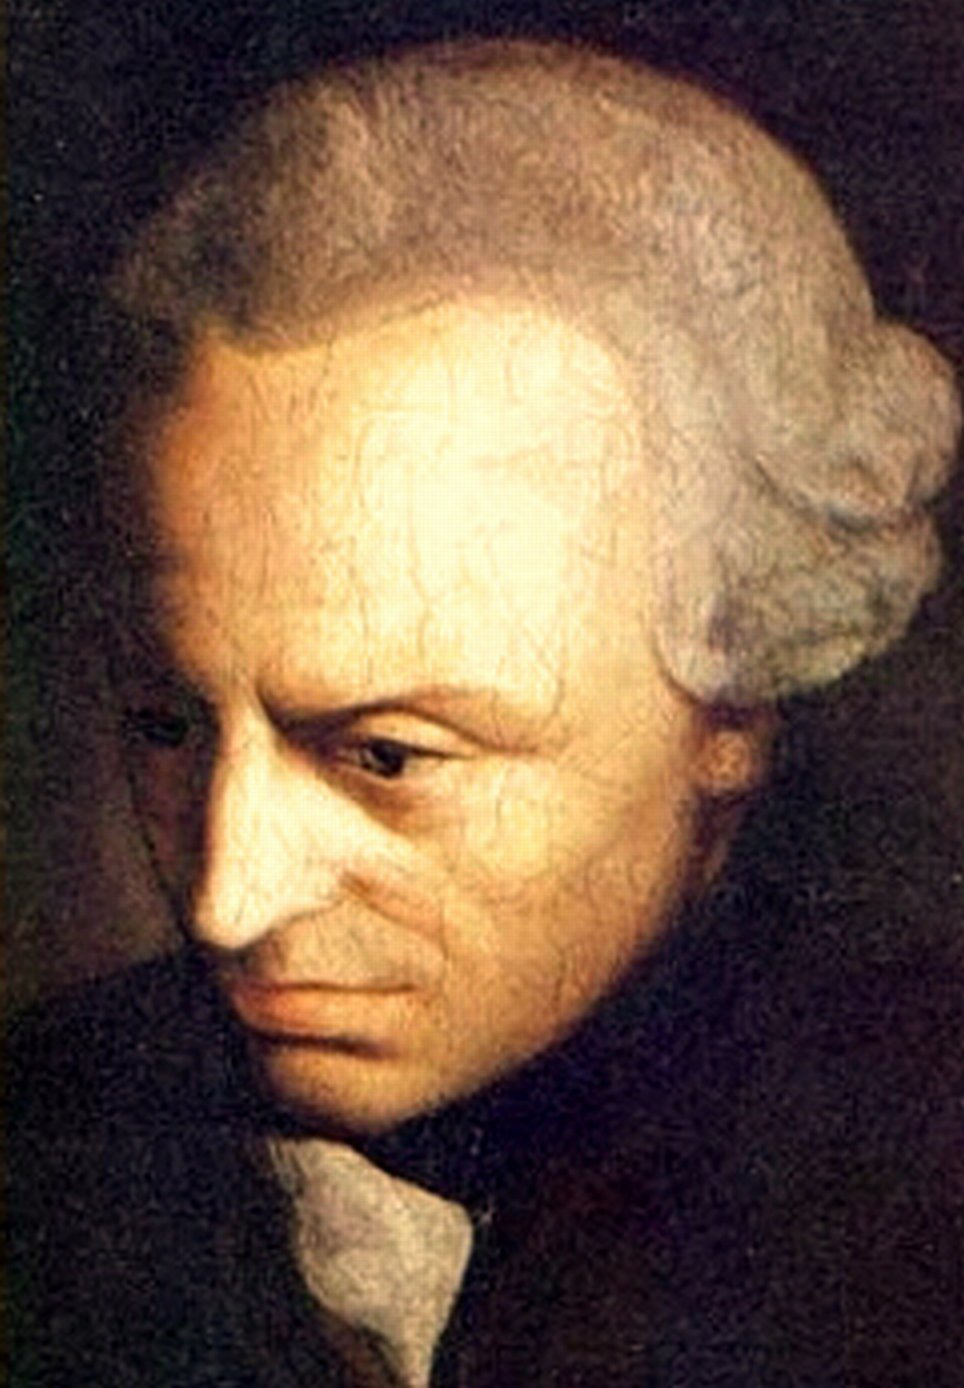
\includegraphics[height=2in]{kant}
\end{figure}


\column{0.65\textwidth}
\begin{figure}[HT]
\begin{block}<2->{Title 1}
	Observation 1 text
\end{block}
\begin{block}<3->{Title 2}
	Observation 2 text
\end{block}
\begin{block}<4->{Conclusion}
	Conclusion
\end{block}

\end{figure}
\end{columns}
\end{frame}

\begin{frame}
\frametitle{Activity}

\begin{figure}[HT]

\begin{block}{Instructions}
\begin{itemize}[]
\item Magnam molestiae quia et quae eum sequi ut. Perferendis facilis eum quaerat unde. Totam rem nulla corrupti. Minima perspiciatis mollitia nulla dolores velit.

\item Quia quam totam placeat voluptas voluptatem cupiditate ut voluptatibus. Non et mollitia fugiat animi doloremque sint odit qui. Dolorem tempore rerum accusantium.

\item Reprehenderit est repudiandae eligendi aperiam sequi quis similique. Doloremque saepe nihil officiis impedit aut sit sit quia. Vel unde ut labore quae.
\end{itemize}
\end{block}
\end{figure}

\end{frame}

\subsection{Middle B2}
\section{Conclusion}
\subsection{Conclusion A}

\begin{frame}
\frametitle{Summary}

\begin{figure}[HT]

\begin{block}{Main Point 1}
	Magnam molestiae quia et quae eum sequi ut. Perferendis facilis eum quaerat unde. Totam rem nulla corrupti. Minima perspiciatis mollitia nulla dolores velit.
\end{block}
\begin{block}{Main Point 2}
Quia quam totam placeat voluptas voluptatem cupiditate ut voluptatibus. Non et mollitia fugiat animi doloremque sint odit qui. Dolorem tempore rerum accusantium.
\end{block}
\begin{block}{Main Point 3}
Reprehenderit est repudiandae eligendi aperiam sequi quis similique. Doloremque saepe nihil officiis impedit aut sit sit quia. Vel unde ut labore quae.
\end{block}
\end{figure}

\end{frame}


\subsection{Conclusion B}

\begin{frame}
\frametitle{Reminders}
\begin{columns}
\column{0.35\textwidth}

\begin{figure}[HT]
\textbf{Weekly To-Dos:}

\begin{block}{}Reading for Wed    \end{block}
\begin{block}{}Reading Quiz       \end{block}
\begin{block}{}Discussion Boards  \end{block}

\end{figure}


\column{0.65\textwidth}
\begin{figure}[HT]
\textbf{Due Dates:}

\begin{block}{Paper Outline}
	Due November 20, 2017 by midnight.
\end{block}
\begin{block}{Paper Final Draft}
	Due December 8, 2017 by midnight.
\end{block}

\end{figure}
\end{columns}

\vspace{0.5cm}

You can get these slides and other helpful materials at: \url{https://blackboard.heartland.edu}

\end{frame}

\end{document}
